\subsection{Measurement Setup}
\label{subsec:04_labMeasurements}

Eleven measurement were taken with five robots on the small-sized \ac{SPL} field
of the HULKs laboratory.
\Cref{fig:04_setup} illustrates the positions of the NAO robots
and the positions of the whistle sound sources.
% -------------------------------------------------------------
\begin{figure}[ht]
	\centering
		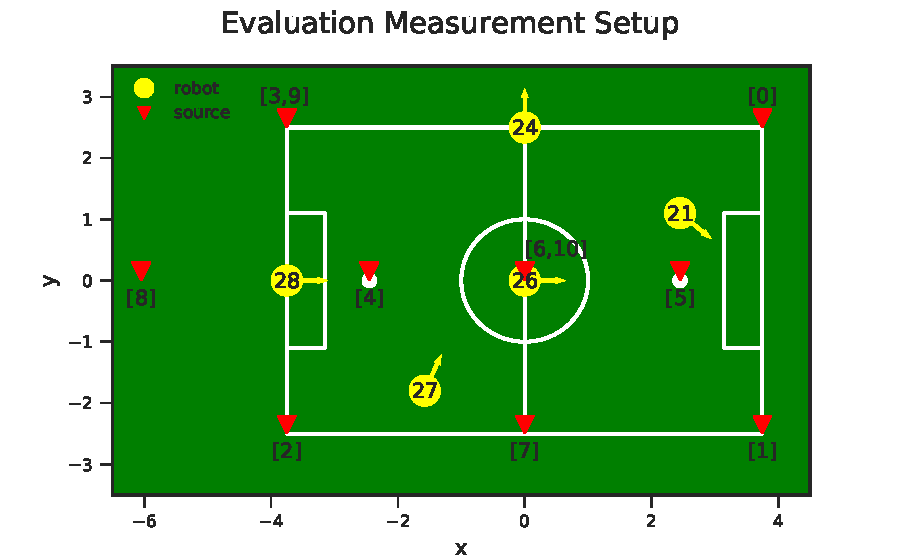
\includegraphics[]{figures/evaluation/setup}
	\caption{Setup of robots and sound source positions for the evaluation measurement.}
    \label{fig:04_setup}
\end{figure}
% -------------------------------------------------------------

According to these, the x- and y-coordinates of the sound source positions and
robots are listed in \cref{tab:04_robots} and \cref{tab:04_sources}, respectively.
Additionally, the positions are named for easier memorability.
The orientation $\theta$ of the robots are defined relatively to the global
x-axis as defined in \cref{subsec:03_coordinates}.
In the following, the measurements introduced in this section are
referred to as \textit{laboratory-dataset}.
% -------------------------------------------------------------
\btline{ht}{1.2}
\btab{|c|c|c|c|}
\hline
NAO & x [\si{m}] & y [\si{m}] & $\theta$ [\si{deg}]\\
\hline
21 & 3.75 & 2.5 & -40.2\\
\hline
24 & 3.75 & -2.5 & 90\\
\hline
26 & 0 & 0 & 0\\
\hline
27 & -3.75 & -2.5 & 66.06\\
\hline
28 & -2.45 & 0 & 0\\
\hline
\etab
\et{Robot positions of the laboratory-dataset}{04_robots}
% -------------------------------------------------------------
\btline{ht}{1.2}
\btab{|c|c|c|c|}
\hline
Measurement & Position Name & x [\si{m}] & y [\si{m}]\\
\hline
0 & front left & 3.75 & 2.5\\
\hline
1 & front right & 3.75 & -2.5\\
\hline
2 & rear right & -3.75 & -2.5\\
\hline
3,9 & rear left & -3.75 & 2.5\\
\hline
4 & own penalty spot & -2.45 & 0\\
\hline
5 & opponent penalty spot & 2.45 & 0\\
\hline
6,10 & center & 0 & 0\\
\hline
7 & center right & 0 & -2.5\\
\hline
8 & behind own goal & -6.05 & 0\\
\hline
\etab
\et{Positions of the whistle sources in the laboratory-dataset}{04_sources}
% -------------------------------------------------------------
